\paragraph{ROM}

\begin{figure}[H]
    \centering
    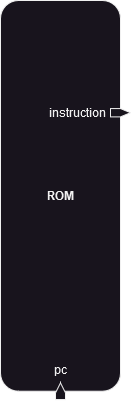
\includegraphics[width=0.20\textwidth]{design/pipelined/rom_ram_reg/images/rom.png}
    \caption{ROM}
    \label{fig:rom}
\end{figure}

The ROM is responsible for storing the program that is being executed by the processor. As its name indicate, it is 
a read-only memory and for the moment it is capable of storing up-to 1024 instructions.

Signals:
\begin{enumerate}[label={\textbullet}]
    \item Input: $pc$, This signal gives the address that needs to be read in the memory.
    \item Output: $instruction$, This signal is representing the instruction that has been read from the ROM.
\end{enumerate}